\documentclass[titlepage, 12pt]{article}

\title{

\includegraphics[width=.3\textwidth]{cvut-logo.jpg}\par
\vspace{10mm}
\indent
\textbf{CZECH TECHNICAL UNIVERSITY IN PRAGUE}

FACULTY OF TRANSPORT SCIENCES

\vfill

{\Large JAN MACEK}
\vspace{10mm}

AGENT-BASED MODELING OF ITS SYSTEMS IN VEHICLE SIMULATOR 
\vspace{15mm}

{\Large DIPLOMA THESIS}
\vfill

}
\date{\Large 2022}

\usepackage[utf8]{inputenc}
\usepackage{listings}
\usepackage{fancyhdr}
\usepackage{graphicx}
\usepackage{parskip}
\usepackage{svg}
\usepackage[a4paper, top=25mm, bottom=25mm, left=30mm, right=20mm, twoside]{geometry}
\usepackage{tabularx}
\usepackage{caption}
\usepackage{hyperref}
\usepackage{xcolor}
\usepackage{amsmath}
\usepackage[sorting=none]{biblatex} 
\usepackage{color}
\usepackage{pdfpages}
\usepackage{enumitem}
\usepackage{amssymb}
\usepackage{booktabs}
\usepackage{microtype}
\usepackage{subfiles}
\usepackage{multirow}

\definecolor{dkgreen}{rgb}{0,0.6,0}
\definecolor{gray}{rgb}{0.5,0.5,0.5}
\definecolor{mauve}{rgb}{0.58,0,0.82}
\definecolor{inline}{rgb}{0.25,0.25,0.80}


\addbibresource{references.bib}

\hypersetup{
    colorlinks,
    linkcolor={red!50!black},
    citecolor={blue!50!black},
    urlcolor={blue!70!black}
}

\pagestyle{fancy}

\graphicspath{{./img}}

\fancyhead[L]{Jan Macek}
\setlength{\headheight}{15pt}

\newlength{\varSepscale}
\setlength{\varSepscale}{16pt}
\newcommand{\itemspacing}[1]{\setlength\itemsep{\dimexpr #1\varSepscale-\varSepscale}}
\newcommand{\term}[1]{\hspace*{2em}\textit{#1}\, -\,}
\newcommand{\rot}[1]{\rotatebox[origin=c]{90}{#1}}
\newcommand{\talign}[3]{\makebox[#2em]{#1\hfill}#3}

%DOCUMENT
\begin{document}
\setlength{\baselineskip}{1.5em}
\maketitle

% 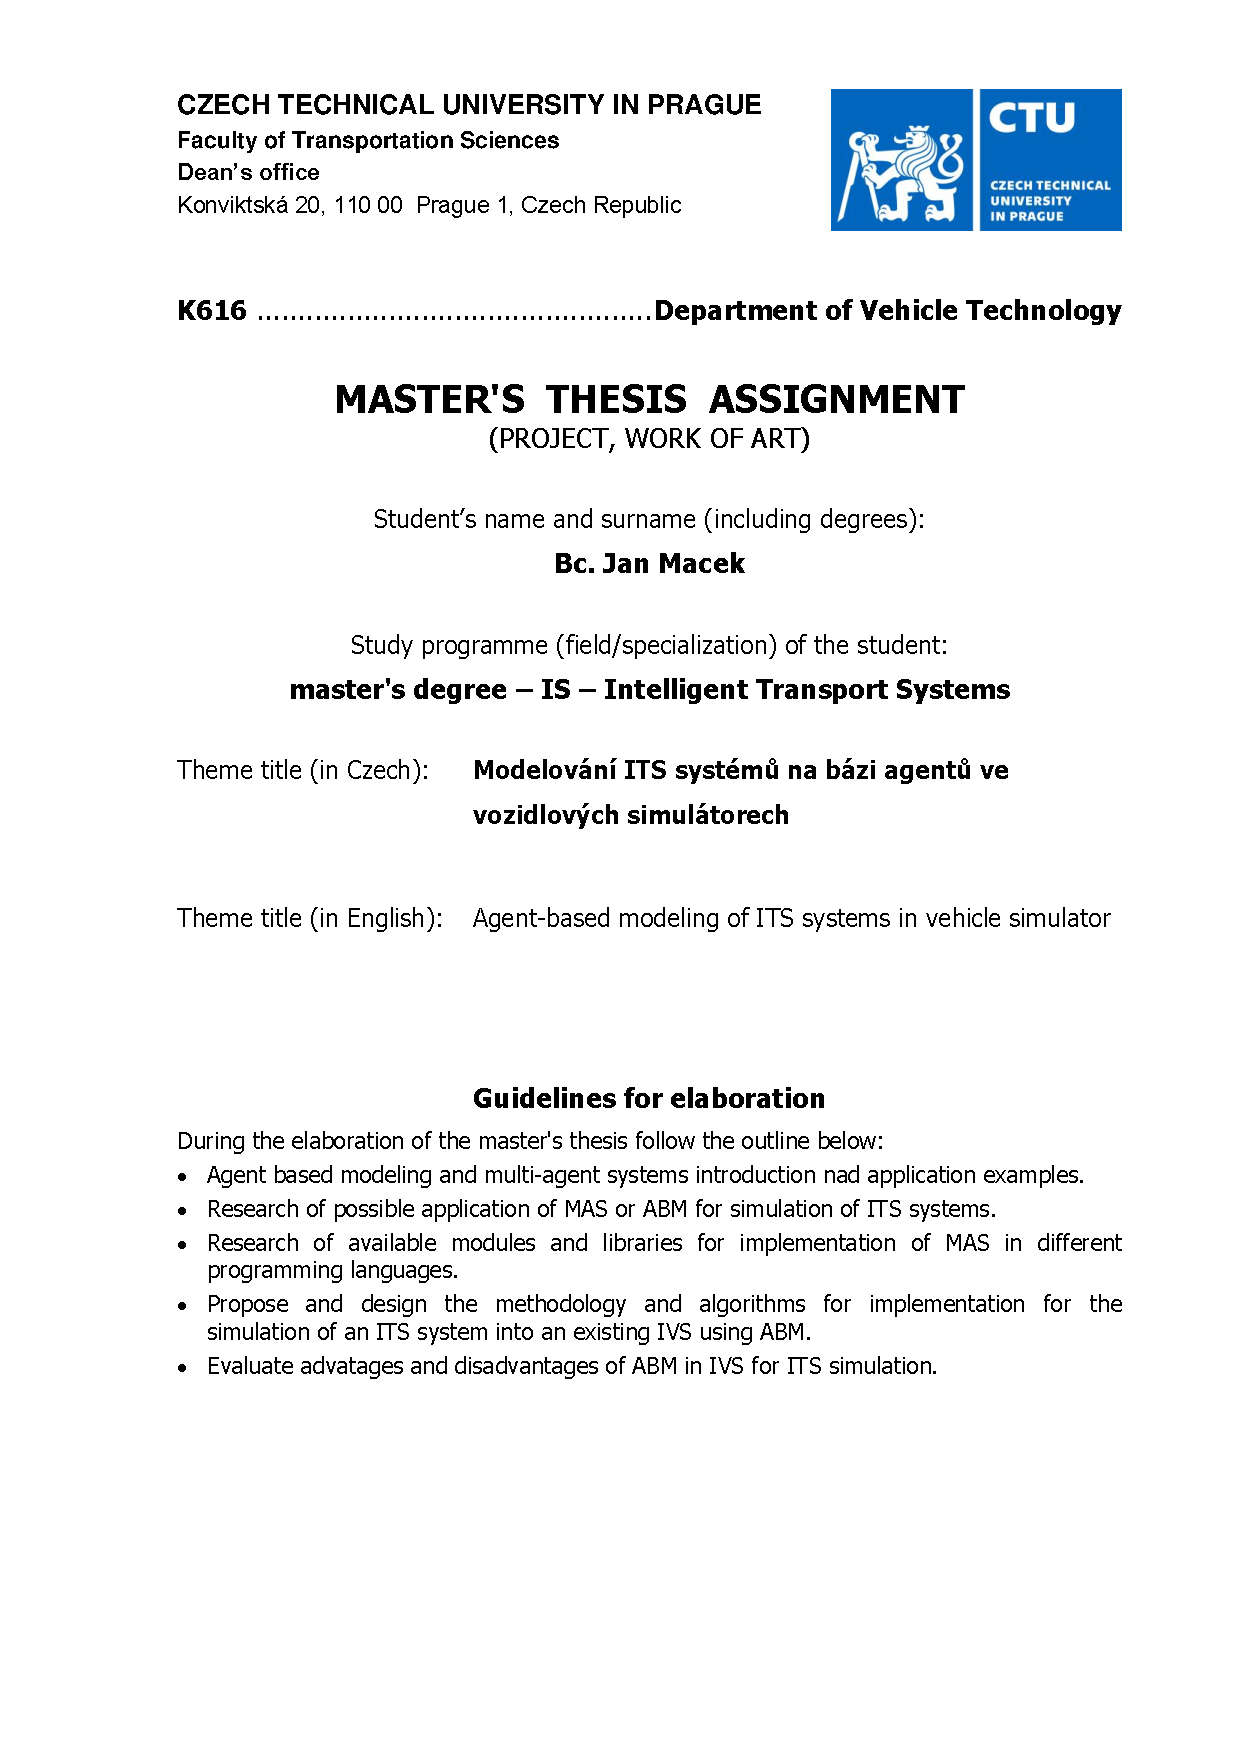
\includepdf[pages=-]{zadani.pdf}

\begin{abstract}
    TODO
\end{abstract}

\tableofcontents
\newpage

\section{Introduction}

In a world in which vehicle transport plays an inseparable role to the society, even with an increasing
demand, it is important to analyze and study driver behaviour and inherently interactions and
relationships between drivers and their surroundings. This is supported by the fact that, even though
substantial advancements in autonomous driving are being made, for the near-future, humans will still
have to control vehicles themselves and therefore be exposed to a substantial risk of danger, as
data shows that about 95 \% of traffic accidents are a result of human error \cite{Parliament2021}. 
Each traffic accident has got a tremendous effect on socio-economic growth. A study be the European
Union states that accident-related expenses (including cost of fatality) cost 1,8 \% of EU GDP \cite{Wijnen2017}.  
A rather non-cynical point of view is that each life lost is a failure in society itself and effort
should be made to diminish fatal accidents.

A method that has proven to be effective at studying driver behaviour and
traffic safety is by using interactive vehicle simulators (IVS), which allow to
undertake experiments in a safe, controlled and reproducible way.  Because
driving simulator is basically a digital twin of a real vehicle, it is naturally
reasonable to make the interaction between the driver and IVS as close to
reality as possible, which inherently improves data quality of the simulation
and potentially also the range of IVS application. An IVS has got a broad
spectrum of employment. It is not only used as a tool to research driver
behaviour, but also used in development and testing of advanced
driver-assistance systems, extending the simulator to a hardware-in-the-loop or
a vehicle-in-the-loop system, which enables to test real hardware and simulate
full road testing.

Simulating the traffic environment is a complex problem, mainly because of
its highly dynamic characteristics. All vehicles  need to interact with
each other and act upon other drivers' actions. Because agent-based simulations
have proven to model complex behaviour well, this modelling technique seems like
a suitable solution for achieving a realistic traffic environment for IVS.

The goal of this thesis is to investigate multi-agent systems, their
characteristics and evaluate usages of these systems, including applications in
the IVS research. Because agent-based systems are also suitable from modelling
communication between entities, research regarding application of the
agent-based systems in relation to ITS systems, which also share the
characteristic of communication and interoperability between individual units
within the system, will also be done.

After investigation of ABM in the IVS and ITS field, an experimental work is presented, which
shows an implementation of a traffic (ITS) system using ABM, with self-proposed
methodology and architecture, which will be described and implemented
into an existing IVS. The proposed simulation system will then be examined and evaluated,
deciding if the implementation was successful, if the systems adequately represent
behaviour observed in real world and possibly performance of the system.

\subfile{its}
\clearpage

\subfile{mas}
\clearpage

\printbibliography
\end{document}
